\documentclass[12pt, titlepage]{article}

\usepackage{fullpage}
\usepackage[round]{natbib}
\usepackage{multirow}
\usepackage{booktabs}
\usepackage{tabularx}
\usepackage{graphicx}
\usepackage{float}
\usepackage{hyperref}
\usepackage{indentfirst}
\hypersetup{
    colorlinks,
    citecolor=black,
    filecolor=black,
    linkcolor=red,
    urlcolor=blue
}
\usepackage[round]{natbib}

\newcounter{acnum}
\newcommand{\actheacnum}{AC\theacnum}
\newcommand{\acref}[1]{AC\ref{#1}}

\newcounter{ucnum}
\newcommand{\uctheucnum}{UC\theucnum}
\newcommand{\uref}[1]{UC\ref{#1}}

\newcounter{mnum}
\newcommand{\mthemnum}{M\themnum}
\newcommand{\mref}[1]{M\ref{#1}}

\title{SE 3XA3: Module Guide\\DNA Says}

\author{Team \#10, Team Name: DNA
		\\ Kareem Abdel Mesih - abdelk2
		\\ John-Paul Dakran - dakranj
		\\ Shady Nessim - nessimss
}

\date{\today}

\begin{document}

\maketitle

\pagenumbering{roman}
\tableofcontents
\listoftables
\listoffigures

\begin{table}[bp]
\caption{\bf Revision History}
\begin{tabularx}{\textwidth}{p{3cm}p{2cm}X}
\toprule {\bf Date} & {\bf Version} & {\bf Notes}\\
\midrule
3/11/2016 & 1.0 & Addition of section 2\\
7/11/2016 & 1.1 & Addition of section 3\\
8/11/2016 & 1.2 & Addition of section 1\\
\bottomrule
\end{tabularx}
\end{table}

\newpage

\pagenumbering{arabic}

\section{Introduction}

\subsection{Overview}
\par This project is a redevelopment of the famous game Simon Says, with a slight modification that makes DNA Says unique while keeping the integrity of the game consistent with the original version. The game consists of three distinct modes - Kareem Says, JP Says and Shady Says.

\subsection{Context}
\par This document consists of the Module Guide (MG) for the project DNA Says. This is the second portion of the design documentation along with the Module Interface Specification (MIS) - which explains the semantics of the code in natural language. \\
\par The Module Guide is a decomposition of the software system into modules. A module is an independent self-contained unit that makes up a complex software system. Decomposing a problem into modules is an extremely important aspect of software design as it promotes the principle of information hiding. Each module is completed concurrently by a programmer and houses a secret of the modules functionality.\\
\par The Module Guide (MG) reveals how the software system will carry out the functionality that is described in the Software Requirements Specification (SRS) document. The potential readers of the document are listed below:
\begin{itemize}
\item Designers/Developers: This document is extremely important for the designers of the software system. It provides a means for the designers to easily identify different parts of the software and relate the implementation to the requirements.
\item New Project Members: This document allows new project members to easily identify the components of the software system. It is a simple way to understand and locate information that relates to specific parts of the software. 
\item Maintainers: 
\end{itemize}

\subsection{Design Principles}

\subsection{Document Structure}


The rest of the document is organized as follows. Section
\ref{SecChange} lists the anticipated and unlikely changes of the software
requirements. Section \ref{SecMH} summarizes the module decomposition that
was constructed according to the likely changes. Section \ref{SecConnection}
specifies the connections between the software requirements and the
modules. Section \ref{SecMD} gives a detailed description of the
modules. Section \ref{SecTM} includes two traceability matrices. One checks
the completeness of the design against the requirements provided in the SRS. The
other shows the relation between anticipated changes and the modules. Section
\ref{SecUse} describes the use relation between modules.

\subsection{Naming Conventions \& Terminology}

\begin{table}[hbp]
\caption{\textbf{Table of Abbreviations}} \label{Table}
\begin{tabularx}{\textwidth}{p{3cm}X}
\toprule
\textbf{Abbreviation} & \textbf{Definition} \\
\midrule
MG & Module Guide\\
SRS & Software Requirements Specification\\
\bottomrule
\end{tabularx}
\end{table}


\begin{table}[!htbp]
\caption{\textbf{Table of Definitions}} \label{Table}
\begin{tabularx}{\textwidth}{p{3cm}X}
\toprule
\textbf{Term} & \textbf{Definition}\\
\midrule
Mode & Different subsections of the game\\
Gantt Chart & Chart outlining the timeline of the project\\
\bottomrule
\end{tabularx}
\end{table}	


\section{Anticipated and Unlikely Changes} \label{SecChange}

This section lists possible changes to the system. According to the likeliness
of the change, the possible changes are classified into two
categories. Anticipated changes are listed in Section \ref{SecAchange}, and
unlikely changes are listed in Section \ref{SecUchange}.

\subsection{Anticipated Changes} \label{SecAchange}

Anticipated changes are the source of the information that is to be hidden
inside the modules. Ideally, changing one of the anticipated changes will only
require changing the one module that hides the associated decision. The approach
adapted here is called design for
change.

\begin{description}
\item[\refstepcounter{acnum} \actheacnum \label{acExecutable}:] The routine that the user follows to start the program. There will be an attempt to create a standalone application rather than require the user to install Python and Pygame.
\item[\refstepcounter{acnum} \actheacnum \label{acInput}:] The main menu.
\item[\refstepcounter{acnum} \actheacnum \label{acInput}:] The flow of the program. There will be a button within each mode to go back to the main menu.
\item[\refstepcounter{acnum} \actheacnum \label{acInput}:] The colours of labels and buttons of the main menu along with all the modes.
\item[\refstepcounter{acnum} \actheacnum \label{acInput}:] The size of the text in each mode.
\end{description}

\subsection{Unlikely Changes} \label{SecUchange}

The module design should be as general as possible. However, a general system is
more complex. Sometimes this complexity is not necessary. Fixing some design
decisions at the system architecture stage can simplify the software design. If
these decision should later need to be changed, then many parts of the design
will potentially need to be modified. Hence, it is not intended that these
decisions will be changed.

\begin{description}
\item[\refstepcounter{ucnum} \uctheucnum \label{ucIO}:] The MVC structure will be transformed to accommodate for the separation of concerns, along with information hiding.
\end{description}

\section{Module Hierarchy} \label{SecMH}

This section provides an overview of the module design. Modules are summarized
in a hierarchy decomposed by secrets in Table \ref{TblMH}. The modules listed
below, which are leaves in the hierarchy tree, are the modules that will
actually be implemented.

\begin{description}
\item [\refstepcounter{mnum} \mthemnum \label{mHH}:] Hardware-Hiding Module*
\item [\refstepcounter{mnum} \mthemnum \label{mHH}:] Main Module
\item [\refstepcounter{mnum} \mthemnum \label{mHH}:] Menu Module
\item [\refstepcounter{mnum} \mthemnum \label{mHH}:] JP Module
\item [\refstepcounter{mnum} \mthemnum \label{mHH}:] Kareem Module 
\item [\refstepcounter{mnum} \mthemnum \label{mHH}:] Shady Module
\item [\refstepcounter{mnum} \mthemnum \label{mHH}:] Setup Module
\item [\refstepcounter{mnum} \mthemnum \label{mHH}:] Update Module
\item [\refstepcounter{mnum} \mthemnum \label{mHH}:] ShowInst Module
\item [\refstepcounter{mnum} \mthemnum \label{mHH}:] ShowScore Module
\item [\refstepcounter{mnum} \mthemnum \label{mHH}:] ShowGoBack Module
\item [\refstepcounter{mnum} \mthemnum \label{mHH}:] DrawKeys Module
\item [\refstepcounter{mnum} \mthemnum \label{mHH}:] FlashKeyAnimation Module
\item [\refstepcounter{mnum} \mthemnum \label{mHH}:] ChangeBackgroundAnimation Module
\item [\refstepcounter{mnum} \mthemnum \label{mHH}:] GameOverAnimation Module
\item [\refstepcounter{mnum} \mthemnum \label{mHH}:] CheckForQuit Module



\end{description}


\begin{table}[H]
\centering
\begin{tabular}{p{0.3\textwidth} p{0.6\textwidth}}
\toprule
\textbf{Level 1} & \textbf{Level 2}\\
\midrule

{Hardware-Hiding Module} & ~ \\
\midrule

\multirow{7}{0.3\textwidth}{Behaviour-Hiding Module} 
& M3\\
& M7\\
& M8\\
& M9\\
& M10\\
& M11\\ 
& M12\\
\midrule

\multirow{3}{0.3\textwidth}{Software Decision Module} 
& M2\\
& M4\\
& M5\\
& M6\\
& M13\\
& M14\\
& M15\\
& M16\\

\bottomrule

\end{tabular}
\caption{Module Hierarchy}
\label{TblMH}
\end{table}
\textbf{Note*:} The Hardware-Hiding Module is not implemented in the hierarchy as there is no hardware involved in this software system.

\section{Connection Between Requirements and Design} \label{SecConnection}

The design of the system is intended to satisfy the requirements developed in
the SRS. In this stage, the system is decomposed into modules. The connection
between requirements and modules is listed in Table \ref{TblRT}.

\section{Module Decomposition} \label{SecMD}

Modules are decomposed according to the principle of ``information hiding''
proposed by \citet{ParnasEtAl1984}. The \emph{Secrets} field in a module
decomposition is a brief statement of the design decision hidden by the
module. The \emph{Services} field specifies \emph{what} the module will do
without documenting \emph{how} to do it. For each module, a suggestion for the
implementing software is given under the \emph{Implemented By} title. If the
entry is \emph{OS}, this means that the module is provided by the operating
system or by standard programming language libraries.  Also indicate if the
module will be implemented specifically for the software.

Only the leaf modules in the
hierarchy have to be implemented. If a dash (\emph{--}) is shown, this means
that the module is not a leaf and will not have to be implemented. Whether or
not this module is implemented depends on the programming language
selected.

\subsection{Hardware Hiding Modules (\mref{mHH})}

\begin{description}
\item[Secrets:]The data structure and algorithm used to implement the virtual
  hardware.
\item[Services:]Serves as a virtual hardware used by the rest of the
  system. This module provides the interface between the hardware and the
  software. So, the system can use it to display outputs or to accept inputs.
\item[Implemented By:] OS
\end{description}

\subsection{Behaviour-Hiding Module}

\begin{description}
\item[Secrets:]The contents of the required behaviours.
\item[Services:]Includes programs that provide externally visible behaviour of
  the system as specified in the software requirements specification (SRS)
  documents. This module serves as a communication layer between the
  hardware-hiding module and the software decision module. The programs in this
  module will need to change if there are changes in the SRS.
\item[Implemented By:] --
\end{description}

\subsubsection{Input Format Module (\mref{mInput})}

\begin{description}
\item[Secrets:]The format and structure of the input data.
\item[Services:]Converts the input data into the data structure used by the
  input parameters module.
\item[Implemented By:] [Your Program Name Here]
\end{description}

\subsubsection{Etc.}


\subsection{Software Decision Module}

\begin{description}
\item[Secrets:] The design decision based on mathematical theorems, physical
  facts, or programming considerations. The secrets of this module are
  \emph{not} described in the SRS.
\item[Services:] Includes data structure and algorithms used in the system that
  do not provide direct interaction with the user. 
  % Changes in these modules are more likely to be motivated by a desire to
  % improve performance than by externally imposed changes.
\item[Implemented By:] --
\end{description}

\subsubsection{Etc.}

\section{Traceability Matrix} \label{SecTM}

This section shows two traceability matrices: between the modules and the
requirements and between the modules and the anticipated changes.

% the table should use mref, the requirements should be named, use something
% like fref
\begin{table}[H]
\centering
\begin{tabular}{p{0.2\textwidth} p{0.6\textwidth}}
\toprule
\textbf{Req.} & \textbf{Modules}\\
\midrule
R1 & \mref{mHH}, \mref{mInput}, \mref{mParams}, \mref{mControl}\\
R2 & \mref{mInput}, \mref{mParams}\\
R3 & \mref{mVerify}\\
R4 & \mref{mOutput}, \mref{mControl}\\
R5 & \mref{mOutput}, \mref{mODEs}, \mref{mControl}, \mref{mSeqDS}, \mref{mSolver}, \mref{mPlot}\\
R6 & \mref{mOutput}, \mref{mODEs}, \mref{mControl}, \mref{mSeqDS}, \mref{mSolver}, \mref{mPlot}\\
R7 & \mref{mOutput}, \mref{mEnergy}, \mref{mControl}, \mref{mSeqDS}, \mref{mPlot}\\
R8 & \mref{mOutput}, \mref{mEnergy}, \mref{mControl}, \mref{mSeqDS}, \mref{mPlot}\\
R9 & \mref{mVerifyOut}\\
R10 & \mref{mOutput}, \mref{mODEs}, \mref{mControl}\\
R11 & \mref{mOutput}, \mref{mODEs}, \mref{mEnergy}, \mref{mControl}\\
\bottomrule
\end{tabular}
\caption{Trace Between Requirements and Modules}
\label{TblRT}
\end{table}

\begin{table}[H]
\centering
\begin{tabular}{p{0.2\textwidth} p{0.6\textwidth}}
\toprule
\textbf{AC} & \textbf{Modules}\\
\midrule
\acref{acHardware} & \mref{mHH}\\
\acref{acInput} & \mref{mInput}\\
\acref{acParams} & \mref{mParams}\\
\acref{acVerify} & \mref{mVerify}\\
\acref{acOutput} & \mref{mOutput}\\
\acref{acVerifyOut} & \mref{mVerifyOut}\\
\acref{acODEs} & \mref{mODEs}\\
\acref{acEnergy} & \mref{mEnergy}\\
\acref{acControl} & \mref{mControl}\\
\acref{acSeqDS} & \mref{mSeqDS}\\
\acref{acSolver} & \mref{mSolver}\\
\acref{acPlot} & \mref{mPlot}\\
\bottomrule
\end{tabular}
\caption{Trace Between Anticipated Changes and Modules}
\label{TblACT}
\end{table}

\section{Use Hierarchy Between Modules} \label{SecUse}

In this section, the uses hierarchy between modules is
provided. \citet{Parnas1978} said of two programs A and B that A {\em uses} B if
correct execution of B may be necessary for A to complete the task described in
its specification. That is, A {\em uses} B if there exist situations in which
the correct functioning of A depends upon the availability of a correct
implementation of B.  Figure \ref{FigUH} illustrates the use relation between
the modules. It can be seen that the graph is a directed acyclic graph
(DAG). Each level of the hierarchy offers a testable and usable subset of the
system, and modules in the higher level of the hierarchy are essentially simpler
because they use modules from the lower levels.

\begin{figure}[H]
\centering
%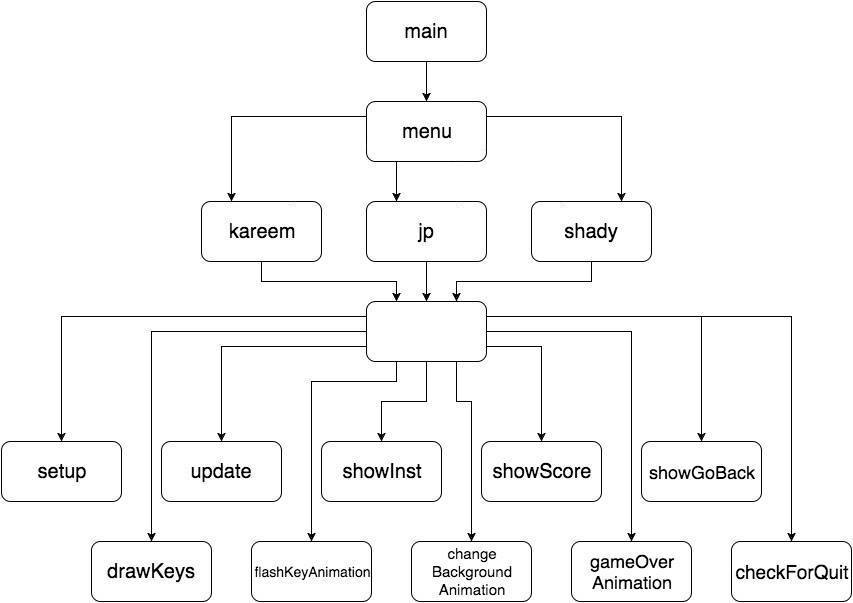
\includegraphics[width=0.7\textwidth]{UsesHierarchy.png}
\caption{Use hierarchy among modules}
\label{FigUH}
\end{figure}

%\section*{References}

\bibliographystyle {plainnat}
\bibliography {MG}

\end{document}